\documentclass[12pt]{article}
\usepackage{enumerate, amsmath, fullpage, hyperref, amsfonts, titlesec, listings, graphicx, enumitem, longtable}
\renewcommand*\contentsname{Table of Contents}
\newlength\tindent
\setlength{\tindent}{\parindent}
\setlength{\parindent}{0pt}
\renewcommand{\indent}{\hspace*{\tindent}}
\lstset{
   breaklines=true,
   basicstyle=\scriptsize\rmfamily}
\begin{document}
\thispagestyle{empty}
\begin{center}
  {\bf\Large Kernel 4}\\
  {\bf\large CS452 - Spring 2014}\\
  Real-Time Programming\vspace{5cm}\\
  {\bf Team }\\
  Max Chen - mqchen\\
  mqchen@uwaterloo.ca\\[1\baselineskip]
  Ford Peprah - hkpeprah\\
  ford.peprah@uwaterloo.ca\vspace{5cm}\\
  Bill Cowan\\
  University of Waterloo\\
  {\bf Due Date:} Monday, $23^{rd}$, June, $2014$
\end{center}
\newpage
% Program Description: how to operate it, full pathname
% Description fo structure of Kernel: algorithms, data structures, etc.
% Location fo source code + MD5
% Output produced by program and explanation of why it does
\thispagestyle{empty}
\tableofcontents
\newpage
\section{Program Description}
\subsection{Getting the Program}
To run the program, one must have read/write access to the source code, as well as the ability to make and run the program.  Before attempting to run the pogram ensure that the following three conditions are met:
\begin{itemize}
  \item You are currently logged in as one of \texttt{cs452}, \texttt{mqchen}, or \texttt{hkpeprah}.
  \item You have a directory in which to store the source code, \\ e.g. \texttt{\textasciitilde/cs452\_microkern\_mqchen\_hkpeprah}.
  \item You have a folder on the FTP server with your username, e.g. \texttt{/u/cs452/tftp/ARM/cs452}.
\end{itemize}
First, you must get a copy of the code.  To to this, log into one of the aforementioned accounts and change directories to the directory you created above (using \texttt{cd}), then run one of
\begin{center}
  \begin{verbatim}
    git clone file:////u8/hkpeprah/cs452-microkern -b kernel4 .
                           or
    git clone file:////u7/mqchen/cs452/cs452-microkern -b kernel4 .
  \end{verbatim}
\end{center}
\vspace{-0.5cm}You will now have a working instance of our kernel4 source code in your current directory.  To make the application and upload it to the FTP server at the location listed above (\texttt{/u/cs452/tftp/ARM/YOUR\_USERNAME}), run \texttt{make upload}.
\\[1\baselineskip]

\subsection{Running the Program}
To run the application, you need to load it into the RedBoot terminal.  Ensure you've followed the steps listed above in the ``Getting the Program'' settings to ensure you have the correct directories and account set up.  Navigate to the directory in which you cloned the source code and run \texttt{make upload}.  The uploaded code should now be located at
\begin{center}
  \texttt{/u/cs452/tftp/ARM/YOUR\_USERNAME/assn4.elf}
\end{center}
To run the application, go to the RedBoot terminal and run the command
\begin{center}
  \texttt{load -b 0x00218000 -h 10.15.167.4 ``ARM/YOUR\_USERNAME/assn4.elf''; go}
\end{center}
The application should now begin by running through the game tasks before reaching a prompt.  The generated files will be located in \texttt{DIR/build} where \texttt{DIR} is the directory you created in the earlier steps.  To access and download an existing version of the code, those can be found at \texttt{/u/cs452/tftp/ARM/mqchen/assn4.elf} and \texttt{/u/cs452/tftp/ARM/hkpeprah/assn4.elf}.
\\
\subsubsection{Bootup Sequence}
Before the program can actually begin accepting input from the user, it has to put the kernel into a state that is ready to begin working.  To this end, the boot sequence of the application does the following sequentially
\begin{enumerate}[label={\bf \arabic*.}, leftmargin=1cm]
  \item Turns on the cache.
  \item Initializes UART2.
  \item Initializes UART1.
  \item Initializes the debugging and display interface.
  \item Initializes the memory.
  \item Initializes the task handling.
  \item Sets up the SWI handler.
  \item Initialzies the logging system.
  \item Turns on the train set.
  \item Writes the display to the screen.
  \item Seeds the pseudo random number generator.
  \item Enables interrupts.
\end{enumerate}
These are done using busy-wait before the application has been running any of the user tasks and moves the kernel into a state ready to begin running tasks.
\\
\subsubsection{Shutdown Sequence}
The application does not terminate until the user issues a shutdown command ('q' on the shell).  The purpose of the shutdown operations is to leave the kernel into a clean state such that another application can be reloaded without having to issue a hardware reboot to the box.  To shutdown, the application busy-waits performing the following tasks sequentially
\begin{enumerate}[label={\bf \arabic*.}, leftmargin=1cm]
  \item Disable interrupts.
  \item Turns off the train set.
  \item Clears any remaining tasks.
  \item Disablees the idle timer.
  \item Dumps the log.
    \\[1\baselineskip]
\end{enumerate}
\subsubsection{Command Prompt}
After the startup tasks have finished running, the user will reach a command prompt where they will be able to enter commands.  A list of available commands the syntax are listed below in the \texttt{Shell} section.
\\[2\baselineskip]

\section{Kernel Structure}

\section{System Primitives}
\begin{longtable}{|l|p{0.3\textwidth}|p{0.5\textwidth}|}
  \hline
  {\bf System Call} & {\bf Prototype} & {\bf Description} \\\hline
  Create & \texttt{int Create(int, void(*)())} & Creates a task with the specified priority to run the given code. \\\hline
  MyTid & \texttt{int MyTid()} & Returns the task ID of the calling task. \\\hline
  MyParentTid & \texttt{int MyParentTid()} & Returns the task ID Of the parent task of the calling task. \\\hline
  Pass & \texttt{void Pass()} & Calling task gives up control to another task of the same priority. \\\hline
  Exit & \texttt{void Exit()} & Calling task exists. \\\hline
  WhoIs & \texttt{int WhoIs(char*)} & Queries nameserver for task ID of task with the given name. \\\hline
  RegisterAs & \texttt{int RegisterAs(char*}) & Registers the given name to the TID of the calling task with the nameserver. \\\hline
  UnRegister & \texttt{int UnRegister(char*)} & Unregister the current task iff its name and tid match what is in the NameServer. \\\hline
  Send & \texttt{int Send(int, void*, int, void*, int)} & Sends a message to the specified task. Blocks on Reply. \\\hline
  Receive & \texttt{int Receive(int*, void*, int)} & Calling task blocks until it receives a message. \\\hline
  Reply & \texttt{int Reply(int, void*, int)} & Replies to the specified task with the given message. \\\hline
  Log & \texttt{int Log(const char*, ...)} & Logs a variable length formatted message to the logger. \\\hline
  Logn & \texttt{int Logn(const char*, n)} & Logs a fixed length message to logger. \\\hline
  AwaitEvent & \texttt{int AwaitEvent(int eventType)} & Blocks until the event identified occurs then returns. \\\hline
  WaitTid & \texttt{int WaitTid(unsigned int tid)} & Waits until the task specified by the \texttt{tid} exits, then returns. \\\hline
  Delay & \texttt{int Delay(int)} & Blocks the current task until the specified number of ticks have elapsed. \\\hline
  DelayUntil & \texttt{int DelayUntil(int)} & Blocks the current task until the specified time has been reached. \\\hline
  Time & \texttt{int Time()} & Returns the current number of ticks that have elapsed. \\\hline
  Getc & \texttt{int Getc(int)} & Returns first unreturned character from the given UART. \\\hline
  Putc & \texttt{int Putc(int, char)} & Transmits the given character to the given UART. \\\hline
  WaitOnSensor & \texttt{int WaitOnSensor(char, unsigned int)} & Blocks the calling task until the specified sensor triggers. \\\hline
  CpuIdle & \texttt{int CpuIdle()} & Returns the percentage of time CPU was idle. \\\hline
  SigTerm & \texttt{void SigTerm()} & Signals to halt the system (kill the NullTask). \\\hline
\end{longtable}
\vspace{1cm}
\subsubsection{Create}
\texttt{Create} creates a new Task Descriptor with the given priority and code, giving it a stack and assigning it an ID.  The created tasks has all the satate needed to run and is added to the priority queues so that it can run the next time it is scheduled.  Returns:
\begin{itemize}
  \item \texttt{tid} - Positive integer id of the newly created task, unique.
  \item $-1$ - if the priority is invalid.
  \item $-2$ - if the kernel is out of task descriptors.
    \\
\end{itemize}
\subsubsection{MyTid}
Returns the task id of the calling task.
\\
\subsubsection{MyParentTid}
Returns the task id of the task that created the calling task.
\begin{itemize}
  \item \texttt{tid} - Positive integer id of the parent task.
  \item $0$ - If task was created by kernel / has no parent.
    \\
\end{itemize}
\subsubsection{Pass}
Moves the calling task from being active back onto the priority queue in a ready-to-run-state.  Has no return value.
\\
\subsubsection{Exit}
Ceases execution of the current task and eliminates it.  Has no return values.
\\
\subsubsection{WhoIs}
Lookup the task with the given name in the NameServer and returns its tid if found.  Does not block waiting for registration.  Returns
\begin{itemize}
  \item \texttt{tid} - Non-negative task identifier on success.
  \item $-1$ - NameServer hasn't been created.
  \item $-2$ - Error  in send.
    \\
\end{itemize}
\subsubsection{RegisterAs}
Register the current task with the name \texttt{name} in the NameServer.  Returns
\begin{itemize}
  \item $0$ - Successfully registered.
  \item $-1$ - NameServer hasn't been created.
  \item $-2$ - Error  in send.
    \\
\end{itemize}
\subsubsection{UnRegister}
Unregister the calling task iff its task ID and name exist in the NameServer.  Does not remove the found task if the tid found at the hash location does not match the tid of the caller.  Returns
\begin{itemize}
  \item $0$ - Successfully unregistered.
  \item $-1$ - NameServer hasn't been created.
  \item $-2$ - Error  in send.
    \\
\end{itemize}
\subsubsection{Send}
On a Send, an \texttt{Envelope\_t} is retrieved from the available pool, and if none are available, an error is returned (A more elegant solution could be implemented by blocking the task until one of structs is available). The msg, msglen, reply, and replylen parameters from the \texttt{Send} call are copied into the respective fields of the \texttt{Envelope\_t}. In addition, the current task pointer is added to the envelope as the sender, and the envelope is set as the outbox pointer of the sender.
\\
The sender is moved to the \texttt{RECV\_BL} state and the envelope is added to the tail of the receiver's inbound message queue, inboxTail.
\\
If the receiver is in the \texttt{SEND\_BL} state, it is added back to the ready queues.
\begin{itemize}
  \item \texttt{size} - Non-negative integer representing the number of bytes copied.
  \item $-1$ - task ID is not possible
  \item $-2$ - task ID does not correspond to a valid task
  \item $-3$ - transaction incomplete
    \\
\end{itemize}
\subsubsection{Receive}
On a Receive, the inbox of the current task is checked. If there is no inbound messages, the task is moved to the \texttt{SEND\_BL} state, and nothing else is done. In this case, the task will be unblocked by Send when a message is actually available, and the user task will have to make another call to Receive to get the message. This process is transparent to the user and is done through the user-mode Receive function.
\\
If there is a message available, then the corresponding values in the envelope are copied into the provided pointers, and the sender task is moved to the \texttt{REPL\_BL} state. The envelope is then removed from the head of the queue so the next message can be received.
\begin{itemize}
  \item \texttt{size} - Non-negative integer representing the number of bytes copied.
    \\
\end{itemize}
\subsubsection{Reply}
For Reply, the intended sender task's outbox parameter is used to find the envelope, and the provided reply message is copied into the provided pointer. The sender is then added back to the ready queue and the envelope is released back into the envelope pool.
\begin{itemize}
  \item \texttt{size} - Non-negative integer representing the number of bytes copied.
  \item $-1$ - task ID is not possible
  \item $-2$ - task ID does not correspond to a valid task
  \item $-3$ - target task is not reply blocked.
    \\
\end{itemize}
\subsubsection{Log}
Allocates a block of memory from the current memory space, and copies the passed string to that location in memory.
\begin{itemize}
  \item $0$ - Successful write
  \item $-1$ - Out of memory from where to write.
    \\
\end{itemize}
\subsubsection{Logn}
Allocates a block of memory from the current memory space, and copies a fixed sized string to that location in memory.
\begin{itemize}
  \item $0$ - Successful write
  \item $-1$ - Out of memory from where to write.
    \\
\end{itemize}
\subsubsection{AwaitEvent}
\texttt{AwaitEvent} blocks until the event identified by the passed integer, \texttt{eventType}, occurs as an interrupt then returns with the value generated by the interrupt.  The value is non-zero.  In the event that the passed integer is not a valid event, it returns $-1$ or if the queues are full it returns $-2$.  Since we do not use event buffers, the previous correspondence for $0$, $-2$ and $-3$ are irrelevant to our implementation.
\\
\subsubsection{WaitTid}
\texttt{WaitTid} blocks on the wait queue of the specified task and returns when that task exists with the status of the exit.  Returns $-1$ if the task does not exist.
\\
\subsubsection{Delay}
Send a message to the ClockServer to block the curren task until the number of ticks have passed.
\\
\subsubsection{DelayUntil}
Send a message to the ClockServer to block the current task until the given number of ticks have been reached.
\\
\subsubsection{Time}
Returns the curren tick count by querying the ClockServer.
\\
\subsubsection{Getc}
Returns the first unreturned character from the given UART; a wrapper for send to the serial IO server.  Blocks until it receives a character.
\begin{itemize}
  \item \texttt{character} - On success returns the read character.
  \item $-1$ - Serial IO server does not exist
  \item $-2$ - Error in send
    \\
\end{itemize}
\subsubsection{Putc}
Queues the given cahracter for trasmission to the specified UART; character may not have been transmitted on return.  Is a wrapper to the IO serial server.
\begin{itemize}
  \item $0$ - On success
  \item $-1$ - Serial IO server does not exist
  \item $-2$ - Error in send
    \\
\end{itemize}
\subsubsection{WaitOnSensor}
Blocks the calling task until the specified sensor has been triggered.  Parameters are passed as \texttt{(module, index)} where index is a positive integer corresponding to the identifier within that module.  Returns
\begin{itemize}
  \item $0$ - On success and unblocked.
  \item $-1$ - If the given sensor does not exist.
    \\
\end{itemize}
\subsubsection{CpuIdle}
Returns the amount of time that the CPU has been idle (running the null task).
\begin{itemize}
  \item \texttt{idle} - Non-negative integer corresponding to the time the CPU has been idle as a fraction of the total CPU time.
    \\
\end{itemize}
\subsubsection{SigTerm}
Tells the Kernel to kill the NullTask and cease execution.  Has no return value.
\\[2\baselineskip]
\section{Algorithms and Data Structures}
\subsection{HashMap/HashTable}
Our HashTable implemented has three attributes:
\begin{enumerate}
  \item \texttt{size} - The size of the array in the HashTable.
  \item \texttt{data} - An array of stored integers that have been hashed to.
  \item \texttt{assigned} - An array indicating whether an index in the array is occupied or not ($1$ for assigned, $0$ unassigned).
\end{enumerate}
And the following functions:
\begin{enumerate}
  \item \texttt{init\_ht(HashTable*)} - Initialize an hashtable by zero'ing out the assigned bits.
  \item \texttt{insert\_ht(HashTable*, char*, int)} - Insert the integer at the hashed index of the char*.
  \item \texttt{exists\_ht(HashTable*, char*)} - Returns $0$ if the hashed index is unassigned, otherwise $1$.
  \item \texttt{lookup\_ht(HashTable*, char*)} - Returns the value stored at the hashed index.  Will return $0$ if the hashed index is unassigned, thus a user should check \texttt{exists\_ht} before calling for a lookup.
  \item \texttt{delete\_ht(HashTable*, char*)} - Delete what is pointed to by the hashed index.  Does nothing if it is unassigned.
    \\[1\baselineskip]
\end{enumerate}
\subsection{Randomization}
To implement randomization, we used the Mersenne Twister algorithm for our psuedorandom number generator, as it is a common generator for random numbers, and will guarantee us a deterministic output provided we know the current index in the twister array.  Random numbers can be generated by calling either \texttt{random()} or \texttt{random\_range(lower\_bound, upper\_bound)} from either the user or kernel structure.
\begin{enumerate}
  \item Populates array with initial values.
  \item Randomizes all items in the array.
  \item Generates and returns random value at index.
  \item Increments to next index.
    \\[1\baselineskip]
\end{enumerate}

\section{Nameserver}
NameServer uses a hash map as the data structure to store the tids in; using the names passed by the registering tasks as the keys to hash with.  It acts as a global lookup table for tasks to find other tasks.  The tid of NameServer is determined at run time by it assigning a value to a global variable within the file and externed through the header files.  It implements three primitives: \texttt{RegisterAs}, \texttt{UnRegister} and \texttt{WhoIs} that have been listed above.
\\
\subsection{NameServer Lookup}
To implement lookup to allow the NameServer to register and identify tasks by name, a HashMap (mentioned in the section above) was used.  To add items to the hash map we needed to convert the string names into integers.  To do this, we used the \texttt{djb2} hashing algorithm.  We ignore collisions as this is a closed space in which we can ensure there will never be a collision.
\begin{enumerate}
  \item String is hashed, which is bounded by $O(n)$ where $n$ is the length of the string.
  \item Lookup in the hash table is $O(1)$ at this point, by accessing the element in the array at the index generated by the hash.
  \item Puts are $O(1)$ by the same methodology.
    \\[2\baselineskip]
\end{enumerate}

\section{ClockServer}
\subsection{Implementation}
The ClockServer registers with the NameServer then creates the ClockNotifier which handles processing of timer generated interrupts.  We use the $508kHz$ $32$-bit timer.  It then writes $5080$ to the timer load register; using the $508kHz$ timer and with $10$ milliseconds, this corresponds to $5080$ in the timer load register.  It then writes to the timer control register to enable it, to set the mode to periodic so that the count resumes back at $5080$ after counting down, and to set the timer to the $508kHz$ timer.  The ClockServer then blocks on \texttt{Receive} to handle messages from other tasks.  When the ClockServer recieves a message of type \texttt{Delay} or \texttt{DelayUntil}, it adds the task to its delay queue sorted by the number of ticks that the task is waiting; the array is sorted in ascending order.  When it receives a message of type \texttt{Tick} it increments its internal counter, replies to the sending task immediately, then iterates through its delay queue waking up every task with a delay less than the current count by replying to them, and stopping as soon as it reaches a task with a delay greater than its current tick count.  This ensures that we do not needlessly check tasks that will not wake up as the queue is sorted.
\\
\subsection{ClockNotifier}
The ClockNotifier is responsible for notifying the ClockServer when a tick occurs; a tick is defined as ten milliseconds passing on the $32$-bit hardware timer.  Since the $508kHz$ clock is used, ten milliseconds is equivalent to setting the value of the clock to $508\cdot 10 = 5080$ upon which it will countdown to $0$ then generate an interrupt.  The ClockNotifier blocks on the timer interrupt and on return it sends a message to the ClockServer indicating a tick took place, which the ClockServer immediately replies to, and then the ClockNotifier blocks on AwaitEvent again.  This task never exits unless the system is shutting down.
\\[1\baselineskip]
\subsection{API}
Implements three primitives: \texttt{Tick}, \texttt{Delay}, and \texttt{DelayUntil} that have been described above.
\\[2\baselineskip]

\section{TrainController}
The TrainController registers with the NameServer and creates a TrainSensorSlave that polls for sensors and awaits characters being transmitted from UART1.  It then blocks on \texttt{Receive} awaiting requests from other tasks that wish to get the state of a sensor, await a sensor being tripped, or for the notifier to message it with the latest sensor data.
\\
\subsection{TrainSensorSlave}
Blocks on \texttt{AwaitEvent} for $10$ characters to be transmitted from UART1 at a time.  Extracts the individual bits from the given characters and sets the status of its sensor to $1$ or $0$ if that sensor tripped (bit value > 0 means that the sensor was tripped).  It then sends the updated results to the TrainController, and repeats the process.
\\[1\baselineskip]
\subsection{API}
The API allows for tasks to wait on sensors by calling \texttt{WaitOnSensor} at which point the calling task is added to that sensors wait queue.  When the sensor is tripped, all the tasks in that queue are unblocked with a return value of $0$.  Tasks may block forever if the sensor never trips.
\\[2\baselineskip]

\section{Shell Task}
\subsection{Commands}
When inputting commands, it is important to note that they must exactly match their prototype or they will be interpreted as garbage by the terminal and equivalent report back \texttt{command: error command not found}.  For example, to move train $1$ at speed $10$, the following command would be entered ``tr 1 10'' followed by a \texttt{RETURN} or \texttt{ENTER}.  All commands must be terminated by a \texttt{RETURN} or \texttt{ENTER} for the terminal to process them.  The syntax for issuing a command is \texttt{``command\_name ARGUMENT\_1 ARGUMENT\_2 .... RETURN''}.  The following table lists the commands supported by this Kernel's shell:
\begin{center}
  \begin{tabular}{|l|l|l|p{0.45\textwidth}|}
    \hline
    {\bf Command} & {\bf Argument 1} & {\bf Argument 2} & {\bf Description} \\\hline
    go   & N/A     & N/A     & Start the train controller (if not started). \\\hline
    stop & N/A     & N/A     & Stop the train controller (if started). \\\hline
    tr   & 1 - 80  & 0 - 14  & Set the train specified by the first argument to the speed specified by the second argument.\\\hline
    ax   & 1 - 80  & 16 - 31 & Run the auxiliary function specified by the second argument on the train specified by the first argument.\\\hline
    rv   & 1 - 80  & N/A     & Reverse the direction of the train specified by the first argument. \\\hline
    li   & 1 - 80  & N/A     & Turn on the lights on the train specified by the first argument. \\\hline
    sw   & 0 - 255 & S or C  & Throw the switch specified by the first argument ot straight (S) or curved (C) specified by the second argument. \\\hline
    ho   & 1 - 80  & N/A     & Turn on the horn on the train specified by the first argument. \\\hline
    add  & 1 - 80  & N/A     & Add a train to the track (useful to introduce new trains to the track). \\\hline
    rps  & N/A     & N/A     & Play a game of Rock-Paper-Scissors. \\\hline
    time & N/A     &         & Reports the current time when the command was called. \\\hline
    q    & N/A     & N/A     & Halt the system and return to RedBoot. \\\hline
  \end{tabular}
  \\[2\baselineskip]
\end{center}
\subsection{Introducing New Trains}
By default, the {\tt TrainUserTask} that listens to the \texttt{Shell} assumes that the trains $45$, $48$, $49$ and $50$ exist on the track to allow the kernel to have some idea of what trains are currently running and where they might be on the track.  Should you wish to use another train that currently is not in the above list, that train can be added to the track by running the \texttt{add} command listed in the above subsection.
\\[1\baselineskip]
\subsection{Shell Display}
The following picture highlights overlay layout of the terminal display:
\begin{figure}[h!]
  \centering
  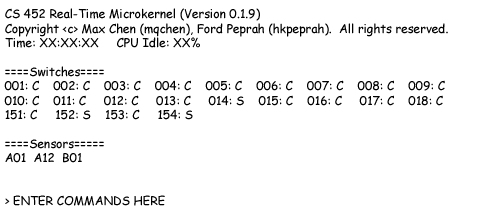
\includegraphics[width=0.9\textwidth]{shell.png}
  \caption{CS452 Microkernel Shell Display}
\end{figure}
Below the top two description lines at the top of the display are the current time (to within $10$ milliseconds) and the percentage of time that the CPU has been idle (calculated as fraction of the time spent doing nothing, running the null task, over the total time the CPU has been running).  Below those two are the current state of the switches ('C' for curved and 'S' for straight), and below those are the recently triggered sensors, read from left to right; the most recent triggered sensor is the farthest left and they scroll horizontally.  Finally, below all of that information is the shell prompt where the user can enter information.
\\[2\baselineskip]
\section{Known Bugs and Errors}
There are known and unknown bugs and errors in our kernel system.  Below we have listed some of the known bugs and errors and grouped them categorically.  Recoverable errors are ones the system can compensate for at runtime in order to correct them and continue the state of the kernel.  Unrecoverable errors are those that would require reprogramming in order to function properly.  Lastly, User Interface Bugs are those tricky bugs that occur due to some configuration of the Kernel and generally do not affect how the application runs, but would affect how the user sees the interface.
\subsection{Recoverable Errors}
\begin{itemize}
  \item Switch $14$ is broken on th second track; to compensate this, the kernel switches it to the straight state which does not cause a derail, though a user could switch it back to curve and allow a derail to become possible again.
\end{itemize}
\subsection{Unrecoverable Errors}
\begin{itemize}
  \item Train derails because of a switch state in the middle switches; in order to remedy this, the train functions should never allow a switch state involving the center switches that would cause a derail.
  \item Known broken switches (e.g. switch $14$ on the second track), and known faulty sensors can cause derails or locations to not accurately be picked up; to compensate for this, the kernel would have to know which sensors are broken and to compensate by looking one sensor ahead or behind that instead to estimate distance.
\end{itemize}
\subsection{User Interface Bugs}
\begin{itemize}
  \item Depending on the state of the box prior to the application being loaded, if the previous group had not exited gracefully, cleared their FIFOs, or otherwise, there may be garbage input read by the IO servers when the kernel is loaded; this is characterized by random printing at the top of the terminal repeatedly that do not seem to be valid characters being typed by the user.  To rectify this issue, reboot the box and reload the program onto it.
  \item During the boot operation, newlines may sometimes be printed erroneously by the terminal causing the display to be printed incorrectly, characterized by a display state not resembling the one listed above in the \texttt{Shell} section.  This can be remedied by quitting the program, and starting it again.
\\[2\baselineskip]
\end{itemize}
\section{MD5 Hashes}
\lstinputlisting{md5}
\end{document}
